\documentclass{beamer}
\usepackage[serbian]{babel}
\usepackage{hyperref}

\usepackage{graphicx}
\graphicspath{ {./../images} }

\title{Speech emotion recognition} 
\subtitle{Računarska inteligencija}

\author{Jelena Keljać, Aleksandra Pešić}
\institute{Matematički fakultet}
\date{Septembar 2022}


\usecolortheme{seahorse}

\begin{document}

\begin{frame}
\titlepage
\end{frame}
    
\begin{frame}
\frametitle{Uvod}
\begin{figure}[t]
\centering
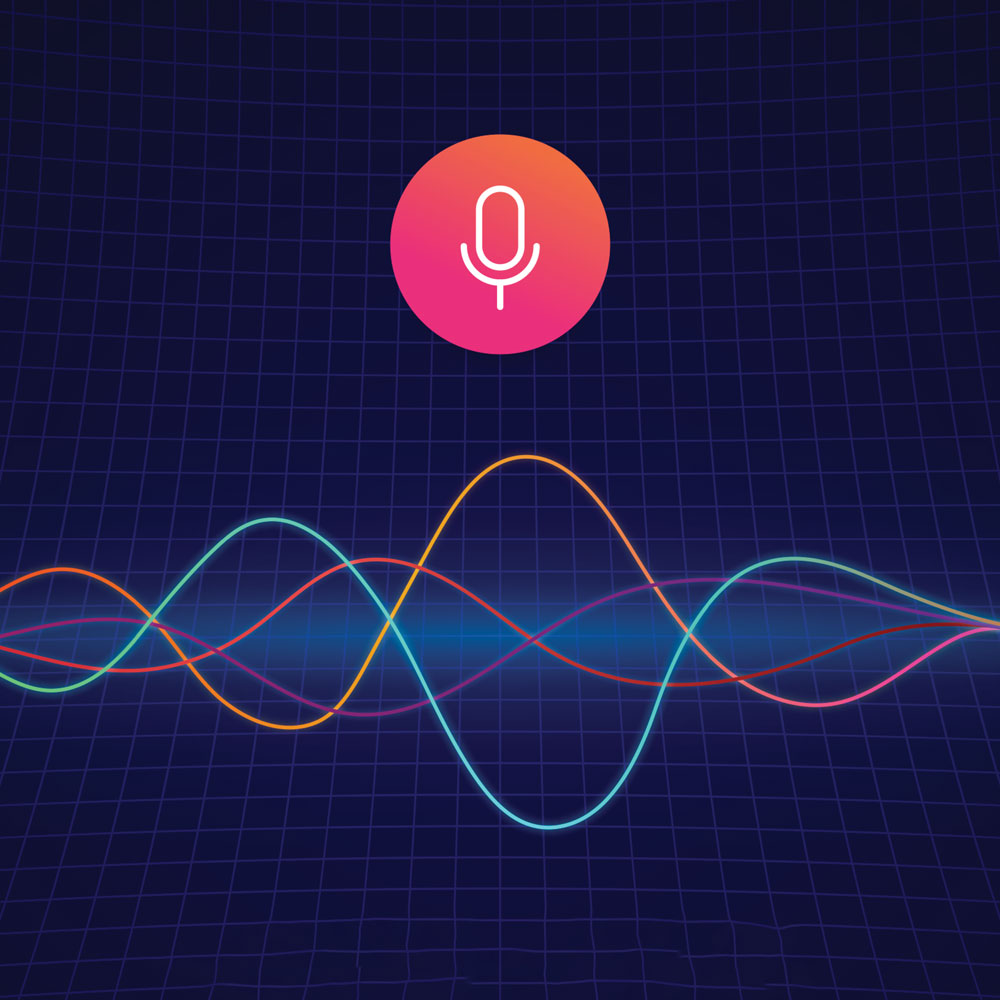
\includegraphics[scale=0.2]{im1.jpg}
\end{figure}
\end{frame}

\begin{frame}{Zvuk}
\begin{itemize}
    \item "Problem" odabira 
    \item MFCC (eng. Mel-frequency cepstral coefficients)
    \item Chroma
    \item Zero-crossing rate
\end{itemize}
\end{frame}

\begin{frame}{MFCC (eng. Mel-frequency cepstral coefficients)}
\begin{itemize}
    \item Predstavlja skup vrednosti, tj. koeficijenata koje sažeto opisuju oblik spektralnog sloja i često se može koristiti za opisivanje boje tona. 
     \item Mel-skala je skala odnosa percipirane frekvencije od strane ljudi sa zapravo izmerenom frekvencijom zvuka.
\end{itemize}
\end{frame}

\begin{frame}{Chroma and Zero cross rate}
\begin{itemize}
    \item Chroma se odnosi na 12 različitih klasa visine tonova i predstavlja intezitet zvuka za svaku od 12 različitih klasa koje predstavljaju 12 različitih polutonova muzičke oktave. 
    \item Stopa prolaska kroz nulu meri koliko puta u određenom vremenskom intervalu je amplituda zvučnog signala prošla kroz vrednost nula.
\end{itemize}
\end{frame}

\begin{frame}{Ulazni podaci}
\begin{itemize}
    \item Za pravljenje našeg modela korišćena su dva seta podataka: 
    \begin{enumerate}
    \item Ryerson Audio-Visual Database of Emotional Speech and Song (Ravdess)
    \item Toronto emotional speech set (Tess)
    \end{enumerate}
    \begin{figure}[h]
    \centering
    
\includegraphics[scale=0.4]{im3.png}
    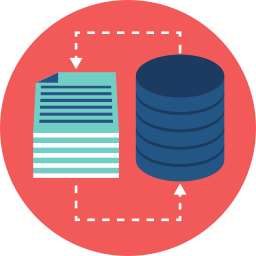
\includegraphics[scale=0.2]{im2.png}
    \end{figure}
    \item librosa.feature.mfcc
\end{itemize}
\end{frame}

\begin{frame}{Model}
    \begin{itemize}
        \item Veštačke neuronske mreže oponašaju biološke neuronske mreže. 
        \item Svaki sloj se sastoji od jedinica, neurona, povezanih sa neuronima iz susednih slojeva težinskim koeficijentima.
        \begin{figure}[h]
        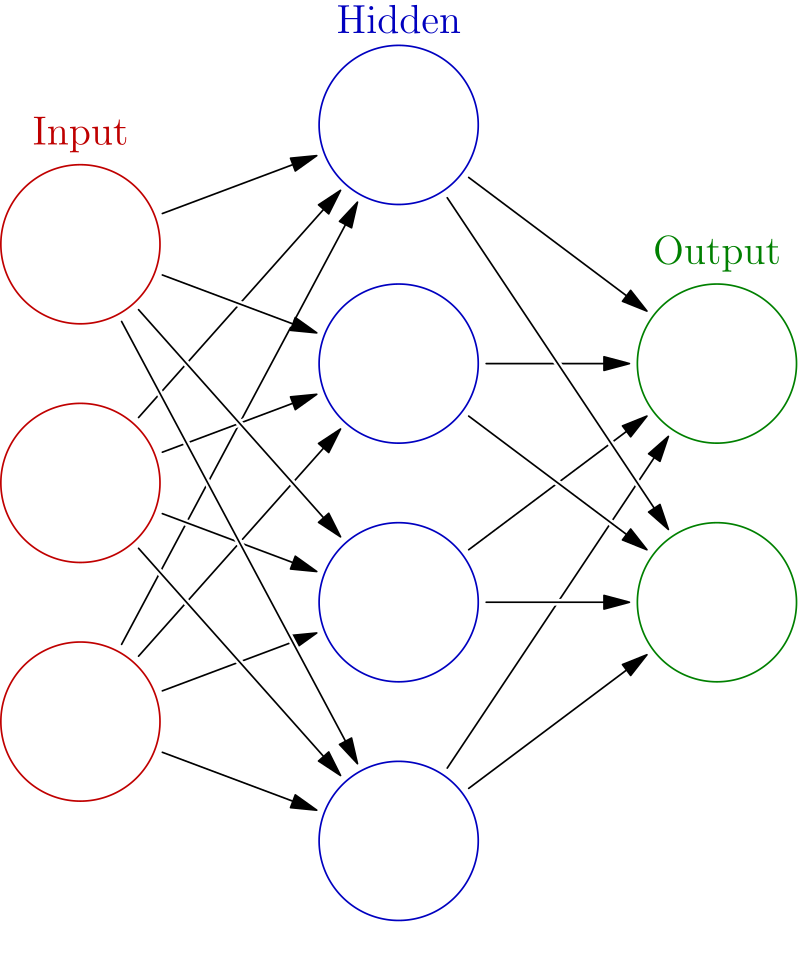
\includegraphics[scale=0.1]{nn.png}
        \end{figure}
        \item sklearn.neural\_network.\textit{MLPClassifier}
        \item tf.keras.\textit{Sequential} 
    \end{itemize}
\end{frame}

\begin{frame}{Rezultati}
Tačnost modela je oko 88\%.
\begin{figure}[t]
\centering
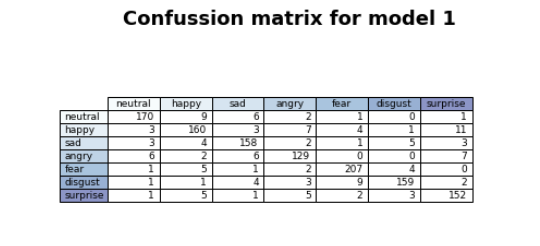
\includegraphics[scale=0.5]{matrix1.png}
\end{figure}    
\end{frame}

\begin{frame}{Rezultati(2)}
Tačnost modela je oko 84\%.
\begin{figure}[t]
\centering
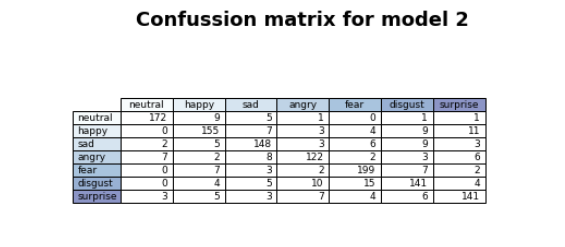
\includegraphics[scale=0.5]{matrix2.png}
\end{figure}    
\end{frame}

\begin{frame}{}
\begin{figure}[h]

\includegraphics[scale=0.3]{end.jpg}
\end{figure}    

\end{frame}


\end{document}
    